\chapter{Asking Texans Their Best Life Advice (Dallas!)}

This School of Hard Knocks interview, rendered here as a companion chapter by LazyingArt LLC through Video2Book, is not a lecture in the usual board-and-equation sense. Still, it has an analytic progression that deserves to be written carefully. James walks through downtown Dallas asking different people the same family of questions: what line of work did you choose, what advice would you give, and what was the best financial decision you ever made? No validated board figures survive for this lecture, so every formula below is a cautious editorial compression of transcript-backed mechanisms rather than a transcription from a visible blackboard. Even with that caution, the structure is clear. Debt can be retired or carried. Assets can appreciate or be missed. Effort can become capacity. Household choices can stabilize a life. Geography can widen the opportunity set. Originality can change the market response.

\section{Dallas as a Field Laboratory}

We begin with a field setting rather than a thesis. James frames the episode as a return to downtown Dallas and as a continuation of an earlier video about millionaires and financial judgment. The opening is brief, but it fixes the governing question that organizes everything that follows: we are going to learn by variation. The same prompt will be put to several lives, and the chapter has to keep the order of those encounters because the order is itself part of the meaning.

That opening also tells us what sort of notes these are. We are not looking for one formal doctrine announced at the beginning and proved at the end. We are moving through a sequence of testimonies, and each one contributes one piece of the mechanism.

\section{Career Formation, Effort, and Debt Discipline}

The first respondent gives the lecture its initial seriousness. The path begins with a degree in psychology, continues through management and information systems, and ends in the ownership of four companies. The implied lesson is not that education is useless, nor that one degree determines one destiny. It is that career formation is often nonlinear, and that entrepreneurship is not purchased merely by possessing a credential.

James then asks for advice to someone who wants to start a business. The answer is severe and very clear: hard work pays off, and the fantasy of owner-level reward with casual owner-level commitment does not survive contact with experience. A compact way to preserve that claim is
\begin{equation}
I \uparrow \Longrightarrow R \uparrow,
\end{equation}
where \(I\) denotes sustained input of time and effort, and \(R\) denotes the results one can plausibly extract. We should not mistake this for a calibrated production function. It is only the lecture's directional rule: if we want business ownership to mean something, we must put in business-owner time.

The first explicit financial mechanism arrives immediately afterward. The best financial decision, says the speaker, was to pay off all credit-card debt and never again rebuild a carried balance. The transcript is slightly garbled at one point, but the mechanism is unmistakable. Let \(D_{\mathrm{cc}}^{(n)}\) be revolving credit-card debt at the start of week \(n\), let \(c_n\) be new charges, and let \(p_n\) be the payment made at settlement. Then
\begin{align}
D_{\mathrm{cc}}^{(n+1)} &= D_{\mathrm{cc}}^{(n)} + c_n - p_n, \\
p_n &= D_{\mathrm{cc}}^{(n)} + c_n
\quad \Longrightarrow \quad
D_{\mathrm{cc}}^{(n+1)} = 0.
\end{align}

\paragraph{Worked update rule.}
This is the most concrete mathematics in the early part of the lecture. We charge during the week, but at settlement we pay the whole carried balance plus the week's new charges. The state update returns the account to zero carried debt:
\begin{equation}
D_{\mathrm{cc}}(t_{\mathrm{settlement}})=0.
\end{equation}
No interest-rate model is needed because the speaker's point is simpler than that. The operative target is not optimized debt; it is no revolving debt.

The same answer is then sharpened by a cash test for extravagant consumption. If \(x\) is the contemplated purchase, \(P_x\) its price, and \(C\) the available cash on hand, then the advice becomes
\begin{equation}
C \ge P_x \Rightarrow \text{buy }x,
\qquad
C < P_x \Rightarrow \text{do not buy }x.
\end{equation}
This is not a universal theorem of personal finance. It is a guardrail. The lecture wants us to see that before we talk about leverage, business creation, or sophisticated investing, we must first know whether we can stop financing extravagance with liabilities.

\section{Technology, Social Skill, and the First Asset Example}

Only after that early discipline does the lecture widen back out into career advice. The next speaker works in IT and says two things at once. Entry is easier now because information is available online; yet that very accessibility does not abolish the need to like the work enough that it does not feel merely like work. We are being told that the expansion of information supply is not the same as the formation of vocation.

The next prompt pushes this even further: what traits matter in a career? The answer is instantaneous and memorable. Social skills matter. Technology, by itself, is not a social skill. This is a useful correction to any account of labor markets that reduces value to credentials and tool familiarity. One still has to persuade, collaborate, present, and function with other human beings.

The sequence then returns to money, but now on the asset side rather than the liability side. A speaker says the best financial decision was buying a house rather than renting, and James asks how much it has appreciated. The answer is about two hundred thousand dollars. If \(V_h(t_0)\) is the value at purchase and \(V_h(t_1)\) the later value, we can preserve the statement as
\begin{equation}
\Delta V_h = V_h(t_1)-V_h(t_0) \approx \text{\$200{,}000}.
\end{equation}

\begin{remark}
This is a self-reported anecdote, not a housing theorem. We are given no basis, no mortgage terms, no maintenance cost, and no holding period. What the lecture wants us to notice is the mechanism: ownership can capture appreciation as household equity, whereas rent does not.
\end{remark}

By this point the first movement of the lecture has taken a definite shape. We begin with nonlinear career formation, pass through effort, move into debt discipline, broaden to employability and social skill, and end with the first numerical illustration of asset ownership.

\section{Risk, Drift, and the Million-Dollar Stress Test}

The next witness is a middle-school counselor, and with that witness the lecture changes register. We are no longer speaking only about accounts and asset values. We are speaking about what sort of person can move through uncertainty without being paralyzed by it. The counselor's most rewarding experience is seeing students grow from children into adults, and that naturally leads to advice for someone entering the real world.

Here the lecture gives us one of its most important tonal beats. The answer begins awkwardly, as if caution were going to be the moral, and then corrects itself: do not be afraid to take a risk. That self-correction matters. The lecture is not praising recklessness. It is exposing the hidden danger in a life that tries never to move outside the safe corridor.

\subsection{Question \& Answer}

\paragraph{Question.}
Is the safe path actually safe?

\paragraph{Answer.}
Not if safety means permanent avoidance of initiative. James sharpens the issue with a stress test: if one had to make a million dollars in a year and life depended on it, what would one do? The answer is comic and desperate at once. There is no constructive plan, only the fantasy of a bank robbery. That is the point. A life organized around avoiding risk can arrive at a moment of pressure with no lawful, disciplined, or imaginative path available. The lecture's answer is therefore not ``be reckless.'' It is: cultivate agency early, so that when pressure comes, you possess more than panic.

That is why this beat belongs exactly where it does. The earlier part of the chapter taught us how not to get trapped by debt. This part asks how not to get trapped by passivity.

The aftershock is immediate and practical. The financial advice to younger people in college is again defensive: do not take loans lightly, and do not open credit cards lightly. The lecture does not abandon prudence after defending risk. It binds the two together. Do not carry needless liabilities, but do not build a whole life on fear of movement.

\section{Self-Investment, the Question of School, and Intentionality}

The Spider-Man segment is a hinge in the lecture, not a novelty inserted for color. The odd-jobs answer is playful, but the financial answer that follows is one of the strongest in the entire episode. The best decision was investing in oneself. Money had previously been spent on things that were ``not it''; the corrective was to spend on oneself, on equipment, and on tools.

A clean notation for that claim is
\begin{equation}
K_{\text{self}} = K_{\text{skills}} + K_{\text{tools}} + K_{\text{equipment}}.
\end{equation}
Here \(K_{\text{self}}\) is editorial shorthand rather than transcript vocabulary, but it preserves the structure exactly. The object of investment is productive capacity.

James then asks whether a college degree is necessary for success in today's society, and the answer is a blunt no. The reason given is equally important: ordinary schooling often prepares people to occupy preset roles, whereas someone who wants to make his own way and leave a legacy must know what he wants and build toward it. The lecture is therefore not simply indulging in anti-school rhetoric. It is moving from skepticism about credentials to a stronger positive demand: intentionality.

\subsection{Question \& Answer}

\paragraph{Question.}
Is college necessary for success?

\paragraph{Answer.}
The lecture gives a cautious practical no, not a universal doctrinal no. Two distinct claims are being made. First, school is not the only route by which value enters a life. Second, if one wants to build something distinctive, a credential cannot substitute for direction. The burden shifts from institutional certification to chosen aim, self-investment, and sustained effort. This is witness testimony, not an econometric law, and the notes should preserve that caution.

The next question to the same speaker makes the constructive side explicit. What would you tell your younger self? The answer is to be intentional about what you want to accomplish. If the goal is clear, the path can be arranged. If the will is scattered, then the path itself becomes scattered. A compact way to record the mechanism is
\begin{equation}
G \text{ clear}
\Longrightarrow
\Pr(\text{goal attainment}) \uparrow.
\end{equation}

\begin{remark}
This is a heuristic arrow, not a quantified estimate. The lecture gives us no decision-theoretic model and no statistics. What it does give us is a strong practical claim: clarity of aim reorganizes conduct.
\end{remark}

The order matters here. We are first told to invest in oneself, then told not to confuse credentialing with destiny, and then told that intention is what converts action into a path. The lecture is now operating at a larger scale than the credit-card example. It is asking how a person becomes economically coherent across years.

\section{Household Architecture: Partner, Family, and Work Ethic}

The next move is one of expansion. A financial decision is no longer just a choice about debt, cash, or an asset purchase. One speaker says the best financial decision was marrying someone with a good financial mind, or more fully, finding a partner with similar aspirations and then spending a lifetime working toward those aspirations together. The lecture here treats alignment itself as a durable economic good.

We should say precisely what kind of claim this is. It is not a return-on-investment theorem for marriage. It is the far broader claim that a household can concentrate effort or dissipate it. Shared aims stabilize long-run action.

The next respondent, a public servant, pushes the category outward once more. The best investment, he says, was investment in the family. The daughters are the proof, and the family is treated as the true object of long-horizon care. Here again the lecture broadens what counts as finance. A life can be organized around liability management, but it can also be organized around people.

Immediately afterward the degree question reappears in a different register. Another speaker says a college degree is not necessary, because a trade and a work ethic can matter more than a piece of paper. This does not erase the earlier answer; it reinforces it. The lecture is widening from credentials to capacities, from capacities to households, and from households to the moral texture of work.

\begin{definition}
In the language of this lecture, a financial decision is any durable choice that shapes future cash flow, future capacity, future alignment, or future opportunity.
\end{definition}

That definition is editorial, but it captures the widening arc of the transcript. What began as budgeting advice is now being treated as life architecture.

\begin{table}
\begin{center}
\begin{tabular}{|l|l|l|}
\hline
Decision type & Representative claim & Main mechanism \\
\hline
Pay off cards & Stop carrying revolving debt & Release cash-flow pressure \\
Cash discipline & Do not finance extravagance & Block liability growth \\
Buy a house & Ownership captured appreciation & Convert price rise into equity \\
Invest in self & Buy tools and build skill & Raise productive capacity \\
Choose partner well & Align aspirations and conduct & Stabilize long-run action \\
Invest in family & Treat household as the project & Build intergenerational strength \\
Learn a trade & Outwork the credential signal & Convert effort into income \\
Relocate & Move where opportunity is thicker & Enlarge the accessible option set \\
Stay low debt & Preserve room to move & Increase optionality \\
Be original & Differentiate the work & Improve market response \\
\hline
\end{tabular}
\end{center}
\end{table}

\section{Geography, Optionality, and Creative Differentiation}

The law-enforcement speaker introduces the next decisive turn. The best financial decision was moving down to Dallas from Mississippi and, with equal emphasis, not spending money on nonsense afterward. Geography enters the chapter not as scenery but as a financial variable. The move is treated as an investment because it changes the density of available opportunity.

A compact shorthand for the speaker's judgment is
\begin{equation}
A(\text{Dallas}) > A(\text{Mississippi}),
\end{equation}
where \(A(L)\) denotes the opportunity set accessible at location \(L\).

\begin{remark}
This is not a measured statistic. It is the transcript's way of saying that the same person, with the same labor and the same ambition, may face a wider opportunity frontier in one place than in another.
\end{remark}

The next respondent turns this place-based idea into a more abstract rule. The best financial decision was paying off debts, not because debt is always bad in principle, but because low debt and high income make movement possible. One can travel, one can relocate, one can invest, one can jump when an opening appears. This is the lecture's clearest account of optionality:
\begin{equation}
D \downarrow,\qquad Y \uparrow
\qquad \Longrightarrow \qquad
O \uparrow,
\end{equation}
where \(D\) is debt burden, \(Y\) is income flow, and \(O\) is practical optionality.

\begin{definition}
Optionality is the usable freedom to move, invest, travel, or change plans when an opportunity presents itself, without first having to unwind a pile of fixed obligations.
\end{definition}

The musician then closes the intellectual arc of the lecture. We are told about collaboration in the studio, about the need to practice, and about the need not to fear one's creativity. The decisive claim is that originality is what people are looking for now. The chapter should preserve this as a market-positioning heuristic:
\begin{equation}
O_r \uparrow \Longrightarrow R_{\text{market}} \uparrow,
\end{equation}
where \(O_r\) denotes originality and \(R_{\text{market}}\) denotes market response.

The transcript contains a slightly garbled line in this part of the interview, but the overall mechanism is plain enough. Practice builds competence, collaboration supplies pressure and feedback, and originality gives the work distinction in a crowded field.

Because no validated frame-backed diagram survives for this lecture, the following figure is explicitly editorial. It summarizes the sequence of mechanisms that the testimonies build together.

\begin{figure}
\begin{center}
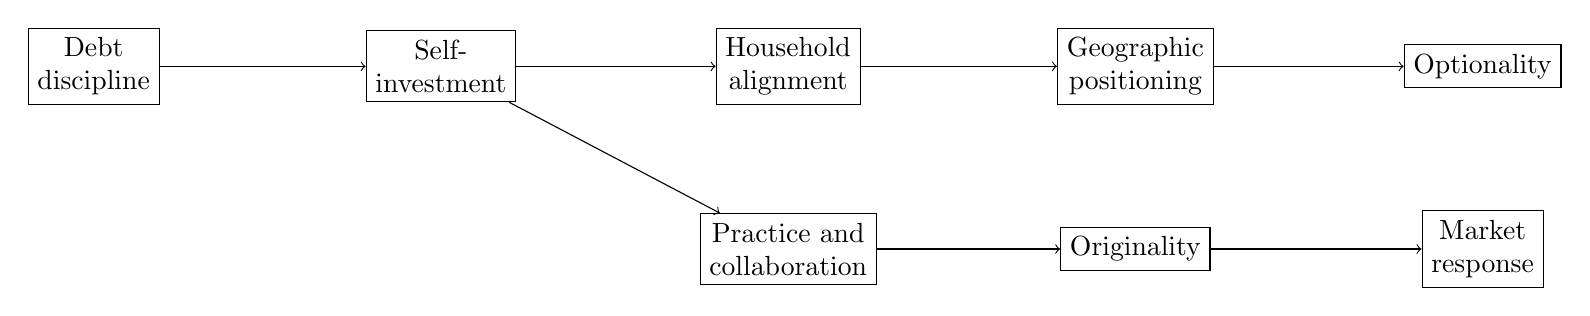
\begin{tikzpicture}[x=2.45cm,y=1.6cm]
\node[draw, rectangle, align=center] (a) at (0,0) {Debt\\discipline};
\node[draw, rectangle, align=center] (b) at (1.8,0) {Self-\\investment};
\node[draw, rectangle, align=center] (c) at (3.6,0) {Household\\alignment};
\node[draw, rectangle, align=center] (d) at (5.4,0) {Geographic\\positioning};
\node[draw, rectangle, align=center] (e) at (7.2,0) {Optionality};

\node[draw, rectangle, align=center] (f) at (3.6,-1.45) {Practice and\\collaboration};
\node[draw, rectangle, align=center] (g) at (5.4,-1.45) {Originality};
\node[draw, rectangle, align=center] (h) at (7.2,-1.45) {Market\\response};

\draw[->] (a) -- (b);
\draw[->] (b) -- (c);
\draw[->] (c) -- (d);
\draw[->] (d) -- (e);

\draw[->] (b) -- (f);
\draw[->] (f) -- (g);
\draw[->] (g) -- (h);
\end{tikzpicture}
\end{center}
\end{figure}

The point of the diagram is not to impose a theory from outside. It is to make visible what the lecture itself does over time. We begin with liabilities, move to capacity, broaden into household structure, then into location and optionality, and finally arrive at differentiated work.

The last advice in the episode is modest but fitting: get more involved with other people in school; learn to be an adult. That ending should not be overlooked. After all the talk of money, trade, debt, and originality, the lecture returns to social formation. One does not build an economic life in a vacuum.

\section{Summary}

The Dallas episode begins as a street interview and ends as a compact theory of practical capital. We begin with work, debt repayment, and refusal of extravagant borrowing. We then widen into technology, social skill, and asset ownership. From there the lecture raises the question of risk, answers it with a demand for agency, and then pushes toward self-investment, skepticism about mere credentialism, and the discipline of intention.

Only after that does the chapter fully broaden into household architecture: partner choice, family, trade, and work ethic. Then the outer frame appears. Location matters. Low debt buys room to move. Creativity is not a luxury add-on but part of the economic mechanism when work is crowded and easy to imitate.

So the chapter closes where the interview itself closes: not with a theorem, but with a sequence of linked rules. Retire the liabilities that pin us down. Convert effort into capacity. Choose a direction and hold it. Build a household that reinforces rather than fragments that direction. Move where the opportunity set is alive. Preserve enough optionality to act when the opening comes. And when the field is crowded, do work that is recognizably your own.